\chapter{Celda Sedra-Ghorab-Martin (R)}

\section{Introducción}

A lo largo de esta sección se centrará en el paper Optimum Congurations
for SingleAmplier Biquadratic Filters, de A. Sedra, M Ghorab y K Martin.
Se parte de la celda propuesta por Deliyannis que se muestra en la
Figura \ref{3_1} y se procede a realizar ciertas transformaciones
(Como la transformación complementaria y la transformación RC) para
llegar a utilizar el circuito propuesto por los autores de este paper.

\begin{figure}[H]
\begin{centering}
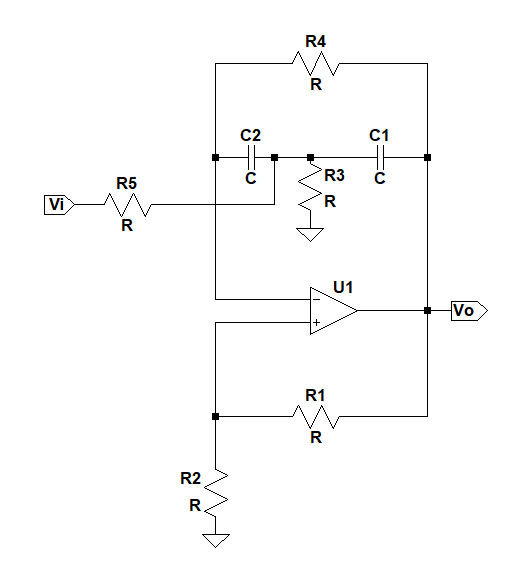
\includegraphics[scale=0.5]{Resources/Deliyannis}
\par\end{centering}
\caption{Circuito Pasabanda Deliyannis}
\label{3_1}

\end{figure}

Como para este Trabajo Práctico se requirió utilizar un filtro pasaaltos,
el circuito propuesto por Sedra-Ghorab-Martin, se muestra en la Figura
\ref{3_2}.

\begin{figure}[H]
\begin{centering}
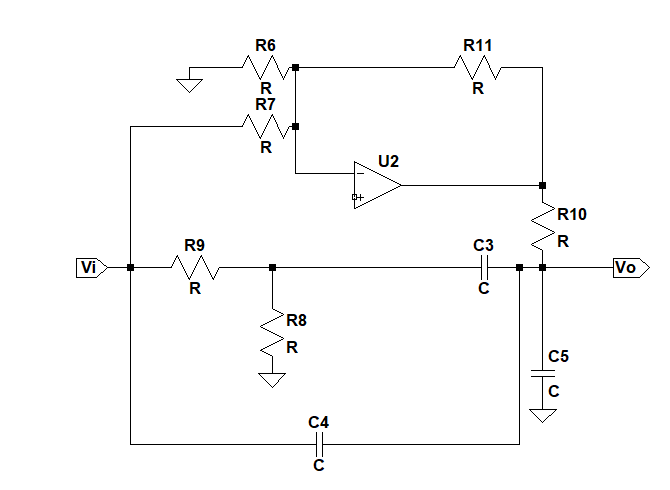
\includegraphics[scale=0.5]{Resources/SedraCir}
\par\end{centering}
\caption{PasaAltos Sedra-Ghorab-Martin}
\label{3_2}

\end{figure}

\section{Diseño}

Primero que nada, para proceder a diseñar se debe tener la plantilla
adecuada a lo que queramos hacer, en nuestro caso, la plantilla propuesta
por la catedra es la que se muestra en el Cuadro \ref{3_c_1}. Siguiendo
el esquema de este PasaAltos, posteriormente se debe utilizar la aproximación
deseada para poder realizar con celdas reales la plantilla.

\begin{table}[H]
\begin{centering}
\begin{tabular}{|c|c|}
\hline 
 & Frecuencia\tabularnewline
\hline 
\hline 
$f_{a}$ & 12.2 (kHz)\tabularnewline
\hline 
$f_{p}$ & 24.4 (kHz)\tabularnewline
\hline 
$A_{a}$ & 40 dB\tabularnewline
\hline 
$A_{p}$ & 2 dB\tabularnewline
\hline 
$\left|Z_{in}(f)\right|$ & $\geq50\,(k\Omega)$\tabularnewline
\hline 
\end{tabular}
\par\end{centering}
\caption{Plantilla del filtro propuesto por la cátedra}
\label{3_c_1}

\end{table}

\subsection{Aproximación eliptica del filtro (Cauer)}

\[
H(s)=\frac{794\cdot10^{-3}s^{4}+102.3\cdot10^{-12}s^{2}+19.3\cdot10^{18}}{s^{4}+308.6\cdot10^{3}s^{3}+110.1\cdot10^{9}s^{2}+8.9\cdot10^{15}s+1.9\cdot10^{21}}
\]

Por lo tanto, reescribiendola de forma que queden 2 transferencias
de orden 2

\[
H_{1}(s)=\frac{794.3\cdot10^{-3}s^{2}+1.8\cdot10^{9}}{s^{2}+284.2\cdot10^{3}s+78.6\cdot10^{9}}
\]

\[
H_{2}(s)=\frac{s^{2}+10.6\cdot10^{9}}{s^{2}+24.4\cdot10^{3}s+24.6\cdot10^{9}}
\]